\documentclass{standalone}
\usepackage{tikz}

\begin{document}

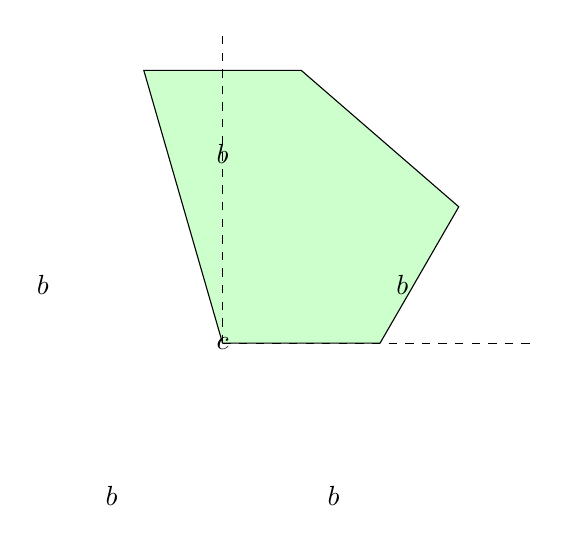
\begin{tikzpicture}[scale=2]
    % Draw the pentagon
    \draw[fill=green!20] (0,0) -- (1,0) -- (1.5,0.866) -- (0.5,1.732) -- (-0.5,1.732) -- cycle;
    
    % Draw the dashed lines
    \draw[dashed] (0,0) -- (2,0);
    \draw[dashed] (0,0) -- (0,2);
    
    % Label the sides of the pentagon
    \foreach \i/\j in {0/b, 1/b, 2/b, 3/b, 4/b} {
        \node at (\i*360/5+90:1.2) {$b$};
    }
    
    % Label the center of the pentagon
    \node at (0,0) {$c$};
\end{tikzpicture}

\end{document}